\chapter{Evaluation}
\label{chap:evaluation}

\section{Goal and Setting}
We evaluate a rule retrieval system used by QA and developers to find and understand Kotlin validation rules. The engine supports three base signals—\emph{Semantic} (embeddings over \texttt{llm\_description}), \emph{BM25} (sparse retrieval over \texttt{keywords}), and \emph{Fuzzy} (string similarity on \texttt{rule\_name})—and a \emph{Hybrid} ranker that linearly combines them.

\paragraph{Dataset.} 30 prompts with a single correct target rule (referenced by name). For each prompt we build a candidate pool as the union of the top–20 from each base signal (deduplicated by \texttt{rule\_id}). Scores from each signal are \emph{per-prompt} normalized to $[0,1]$ before Hybrid combination.

\section{Metrics}
Our primary metric is \textbf{MRR@5} (Mean Reciprocal Rank at cutoff 5):
\[
\mathrm{MRR@5}=\frac{1}{|Q|}\sum_{q\in Q} \frac{\mathbb{1}[r_q\le 5]}{r_q},
\]
where $r_q$ is the rank position of the correct rule for query $q$ (undefined $\Rightarrow 0$).

Secondary metrics are \textbf{Hit@1}, \textbf{Hit@3}, \textbf{Hit@5} (fraction of queries where the correct rule appears in the top $k$) and \textbf{Coverage} (fraction where it appears anywhere in the candidate pool).

\section{Tuning Protocol (LOOCV over the weight simplex)}
The Hybrid score is a convex combination
\[
\text{score} = w_s S_{\text{sem}} + w_b S_{\text{bm25}} + w_f S_{\text{fuzzy}},
\qquad w_s,w_b,w_f\ge 0,\ \ w_s+w_b+w_f=1.
\]
We tune $(w_s,w_b,w_f)$ by \emph{Leave-One-Out Cross-Validation (LOOCV)} over prompts with a simple grid on the 2-simplex (step $0.1$; 66 combinations):
\begin{enumerate}
  \item For each prompt $p$ in the set of 30, hold $p$ out as the validation case.
  \item On the remaining 29 prompts, evaluate all weight triples and select the one with the highest average MRR@5.
  \item Apply that triple to $p$ and record its metrics.
\end{enumerate}
The final LOOCV score is the average over all held-out prompts. We also report the \emph{median} weight triple across folds for interpretability (this is the single set of weights you would ship).

\section{Results}
\subsection{Baselines and Production Hybrid}
Table~\ref{tab:baselines} reports per-method performance; the production Hybrid uses $(w_s,w_b,w_f)=(0.60,0.35,0.05)$.

\begin{table}[h]
\centering
\small
\begin{tabular}{l S[table-format=1.6] S[table-format=1.6] S[table-format=1.6] S[table-format=1.6] S[table-format=1.6]}
\toprule
\textbf{Method} & \textbf{MRR@5} & \textbf{Hit@1} & \textbf{Hit@3} & \textbf{Hit@5} & \textbf{Coverage} \\
\midrule
BM25           & 0.387821 & 0.307692 & 0.461538 & 0.500000 & 0.884615 \\
Semantic       & 0.440385 & 0.269231 & 0.576923 & 0.730769 & 0.884615 \\
Fuzzy          & 0.241667 & 0.192308 & 0.269231 & 0.346154 & 0.884615 \\
\addlinespace
Hybrid (prod)  & 0.433974 & 0.346154 & 0.500000 & 0.576923 & 0.884615 \\
\bottomrule
\end{tabular}
\caption{Baselines and production Hybrid.}
\label{tab:baselines}
\end{table}

\subsection{Hybrid Tuning (LOOCV)}
LOOCV over the weight grid improves the Hybrid to the scores in Table~\ref{tab:loocv}. The tuned LOOCV performance is \emph{not} the same calculation as evaluating a single fixed weight set on all prompts; it averages per-fold held-out performance, which is stricter and avoids overfitting.

\begin{table}[h]
\centering
\small
\begin{tabular}{l S[table-format=1.6] S[table-format=1.6] S[table-format=1.6] S[table-format=1.6] S[table-format=1.6]}
\toprule
\textbf{Method} & \textbf{MRR@5} & \textbf{Hit@1} & \textbf{Hit@3} & \textbf{Hit@5} & \textbf{Coverage} \\
\midrule
Hybrid (tuned, LOOCV) & 0.482051 & 0.307692 & 0.615385 & 0.807692 & 0.884615 \\
\bottomrule
\end{tabular}
\caption{LOOCV-tuned Hybrid performance.}
\label{tab:loocv}
\end{table}

\paragraph{Median tuned weights.} Across folds, the median optimal weights are:
\[
\boxed{(w_s,w_b,w_f) = (0.80,\ 0.10,\ 0.10)}.
\]
These median weights are used for ablation and sensitivity analyses below (a single, shippable configuration). Evaluating this single configuration on the full dataset (not LOOCV) yields a center MRR@5 of $0.526923$; the difference vs.\ Table~\ref{tab:loocv} is expected because LOOCV tests each prompt with weights learned \emph{without} seeing that prompt.

\subsection{MRR@5 Comparison Plot}
\begin{figure}[h]
\centering
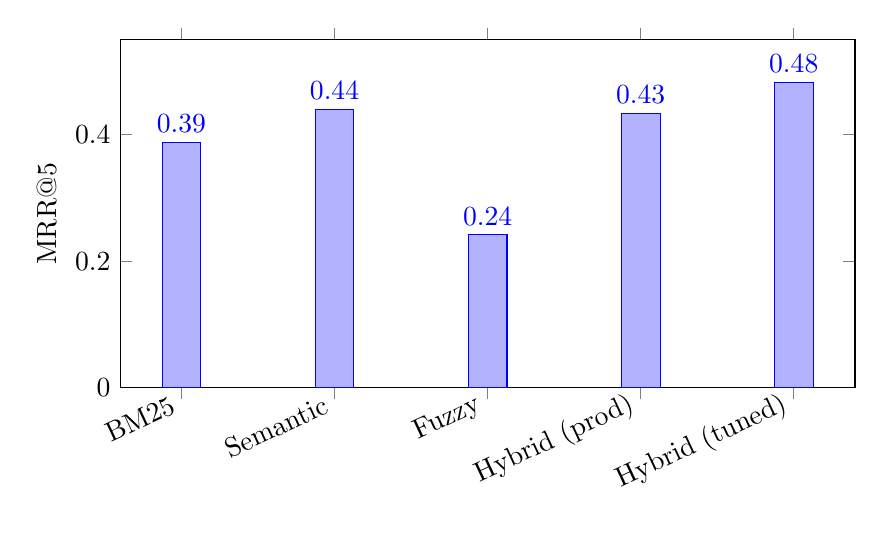
\begin{tikzpicture}
\begin{axis}[
    ybar,
    bar width=14pt,
    ymin=0, ymax=0.55,
    ylabel={MRR@5},
    symbolic x coords={BM25,Semantic,Fuzzy,Hybrid (prod),Hybrid (tuned)},
    xtick=data,
    xticklabel style={rotate=25,anchor=east},
    width=0.9\textwidth,height=6cm,
    nodes near coords,
    nodes near coords align={vertical},
]
\addplot coordinates {(BM25,0.387821) (Semantic,0.440385) (Fuzzy,0.241667) (Hybrid (prod),0.433974) (Hybrid (tuned),0.482051)};
\end{axis}
\end{tikzpicture}
\caption{MRR@5 comparison across methods (LOOCV result for tuned Hybrid).}
\label{fig:mrr_bar}
\end{figure}

\subsection{Ablation Study (Median Weights)}
Starting from the median tuned Hybrid weights $(0.8,0.1,0.1)$, we remove one signal at a time (setting its weight to zero and renormalizing). Results in Table~\ref{tab:ablation} show that Semantic contributes most, BM25 helps, and Fuzzy has the smallest impact—but still provides a positive effect in the median configuration.

\begin{table}[h]
\centering
\small
\begin{tabular}{l S[table-format=1.6] S[table-format=1.6] S[table-format=1.6] S[table-format=1.6]}
\toprule
\textbf{Configuration} & \textbf{MRR@5} & \textbf{Hit@1} & \textbf{Hit@3} & \textbf{Hit@5} \\
\midrule
No Semantic & 0.393590 & 0.346154 & 0.423077 & 0.500000 \\
No BM25     & 0.444872 & 0.307692 & 0.576923 & 0.730769 \\
No Fuzzy    & 0.521795 & 0.384615 & 0.692308 & 0.769231 \\
\bottomrule
\end{tabular}

\vspace{0.25em}
\small Coverage is $0.884615$ for all three settings.
\caption{Ablation starting from median tuned Hybrid (single fixed weights).}
\label{tab:ablation}
\end{table}

\subsection{Sensitivity Analysis (Median Weights)}
We vary one weight by $\Delta\in\{-0.20,-0.10,0,+0.10,+0.20\}$ (clipped to $[0,1]$ and renormalized) and re-evaluate MRR@5. The curves are reproduced exactly from the notebook in Figure~\ref{fig:sensitivity}.

\begin{figure}[h]
\centering
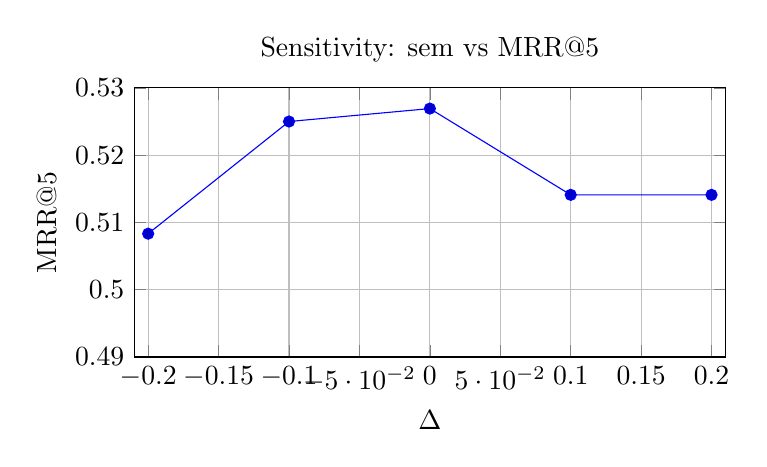
\begin{tikzpicture}
\begin{axis}[
    title={Sensitivity: sem vs MRR@5},
    xlabel={$\Delta$}, ylabel={MRR@5},
    width=0.75\textwidth, height=5cm, grid=both, xmin=-0.21, xmax=0.21, ymin=0.49, ymax=0.53
]
\addplot+[mark=*] coordinates {(-0.20,0.508333) (-0.10,0.525000) (0.00,0.526923) (0.10,0.514103) (0.20,0.514103)};
\end{axis}
\end{tikzpicture}

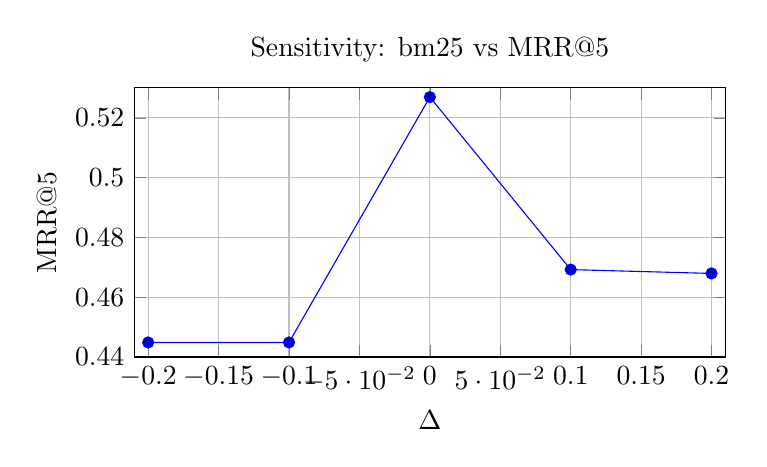
\begin{tikzpicture}
\begin{axis}[
    title={Sensitivity: bm25 vs MRR@5},
    xlabel={$\Delta$}, ylabel={MRR@5},
    width=0.75\textwidth, height=5cm, grid=both, xmin=-0.21, xmax=0.21, ymin=0.44, ymax=0.53
]
\addplot+[mark=*] coordinates {(-0.20,0.444872) (-0.10,0.444872) (0.00,0.526923) (0.10,0.469231) (0.20,0.467949)};
\end{axis}
\end{tikzpicture}

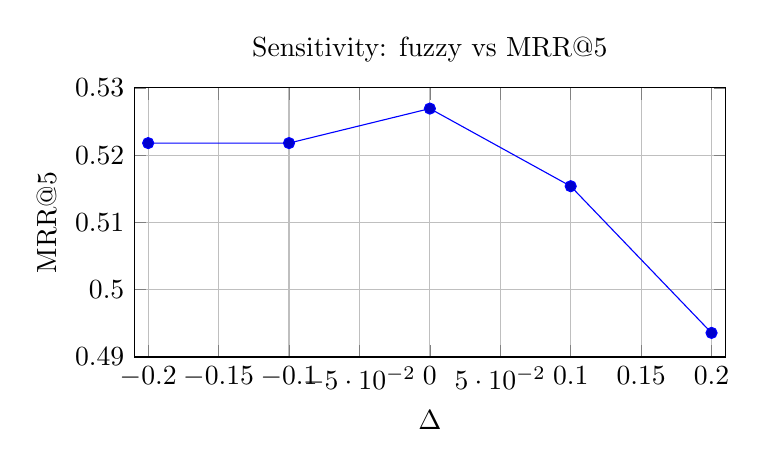
\begin{tikzpicture}
\begin{axis}[
    title={Sensitivity: fuzzy vs MRR@5},
    xlabel={$\Delta$}, ylabel={MRR@5},
    width=0.75\textwidth, height=5cm, grid=both, xmin=-0.21, xmax=0.21, ymin=0.49, ymax=0.53
]
\addplot+[mark=*] coordinates {(-0.20,0.521795) (-0.10,0.521795) (0.00,0.526923) (0.10,0.515385) (0.20,0.493590)};
\end{axis}
\end{tikzpicture}
\caption{Sensitivity of MRR@5 to $\pm 0.2$ per-weight perturbations (median tuned weights baseline at $\Delta=0$).}
\label{fig:sensitivity}
\end{figure}

\section{Interpretation}
\paragraph{Effectiveness.} The tuned Hybrid (LOOCV) improves MRR@5 from $0.433974$ (production) to $0.482051$ (\,+4.81\,pp absolute), with strong gains in early precision (Hit@3: $0.50\rightarrow0.615$; Hit@5: $0.577\rightarrow0.808$). Coverage stays constant at $0.885$, indicating the candidate pool is already sufficiently broad.

\paragraph{Role of signals.} Semantic is the strongest individual signal (MRR@5 $=0.440$) and dominates the tuned combination. BM25 contributes complementary lexical grounding (its removal reduces performance relative to the full median configuration). Fuzzy alone is weak, but in the hybrid its weight can be kept small and safely adjusted.

\paragraph{Robustness.} Sensitivity curves show a broad plateau around the median weights; small perturbations ($\pm 0.1$–$0.2$) do not collapse performance, which is desirable for maintainability.

\paragraph{On LOOCV vs.\ single fixed weights.} LOOCV reports held-out performance per prompt and thus is more conservative (MRR@5 $=0.482$). Evaluating the \emph{single} median weight vector on the entire dataset (the setting used for ablation/sensitivity) gives a higher center score ($0.527$), as it is not cross-validated. Both are reported to transparently separate generalization from point estimates.

\section{Takeaways}
\begin{itemize}
  \item The Hybrid ranker outperforms any single signal; tuning via LOOCV delivers meaningful gains on developer-centric metrics.
  \item A practical, shippable weight setting is \textbf{$(w_s,w_b,w_f)=(0.80,0.10,0.10)$}.
  \item Future work: expand the dataset, consider graded labels for nDCG, and explore light neural re-ranking while retaining the same evaluation protocol.
\end{itemize}
